%% Manuscript for Electric Power Systems Research (Elsevier)
%% Based on elsarticle-template-harv.tex from the EPSR LaTeX bundle.
%% EPSR uses name-year (Harvard) citations: \citet{key} -> Author (Year),
%% \citep{key} -> (Author, Year). References come from refs.bib.
%%
%% Word limit (Full Length Article): 7000 words, counting abstract, text,
%% tables, figure captions and appendices. References and acknowledgements
%% are not counted. State the article length in the cover letter.

\documentclass[preprint,review,12pt,authoryear]{elsarticle}

\usepackage{epsr}
\usepackage{amssymb}
\usepackage{amsmath}
\usepackage{booktabs}
\usepackage{tabularx}   % tables that fit \textwidth and wrap long cells
\usepackage{flafter}    % a float never appears before the text that calls it
\usepackage{siunitx}
\usepackage[hidelinks]{hyperref}
%% Line numbers help reviewers cite exact lines. Uncomment \linenumbers to switch them on.
\usepackage{lineno}
%\linenumbers

\journal{Electric Power Systems Research}

\begin{document}

\begin{frontmatter}

\title{Day-ahead probabilistic forecasting of residential rooftop photovoltaic power: transfer to unseen systems and the input-imposed accuracy limit}

\author[mit]{Chandradip Roy\corref{cor1}}
\ead{official.chandradip@gmail.com}
\cortext[cor1]{Corresponding author.}

\author[dtsc]{Sara Ghane}
\ead{sara.ghane@dtsc.be}

\affiliation[mit]{organization={Manipal Institute of Technology},
            addressline={Udupi-Karkala Rd, Eshwar Nagar},
            city={Manipal},
            postcode={576104},
            state={Karnataka},
            country={India}}

\affiliation[dtsc]{organization={The Belgian Research Lab for AI in INdustry (BRAIN), DT Services and Consulting},
            country={Belgium}}

\begin{abstract}
Day-ahead photovoltaic (PV) forecasts for individual rooftops support household energy management, aggregator bidding and distribution-grid operation, but reported accuracy gains rarely show how close they are to a limit. We diagnose that limit for 33 residential rooftops in Belgium at 15-min resolution over 26 months, with operational numerical weather prediction (NWP) issued one day ahead. Four tests agree. Adding the measured output of every other rooftop, a proxy for perfect regional weather knowledge, raises $R^2$ by only 0.023. Residual autocorrelation falls from 0.72 at 15 min to 0.015 at 24 h, the signature of displaced cloud rather than correctable bias. Irradiance forecast error varies by 3.3\% across rooftops spread over $180 \times 210$ km. Model output statistics that remove 73\% of the systematic irradiance bias change forecast power by less than 0.0005 in $R^2$. Two methodological results generalise. Scoring the forecast against ERA5, a reanalysis from the same centre, understates its RMSE by a factor of 1.69 and reverses the sign of its bias. Hyperparameters selected on a chronological split transfer poorly to unseen rooftops, and selecting them against held-out systems halves the failure rate. An unseen rooftop receives median $R^2$ 0.704, against 0.811 pooled over rooftops seen in training, and transfer failure follows installation metadata: the observed-to-nameplate capacity ratio correlates with forecast bias at +0.709.

\end{abstract}

%% Graphical abstract is optional for EPSR; leave empty unless one is prepared.
%% \begin{graphicalabstract}
%% \includegraphics{grabs}
%% \end{graphicalabstract}

\begin{highlights}
%% Elsevier highlights: 3-5 bullets, max. 85 characters each including spaces.
\item Perfect regional weather knowledge adds only 0.023 $R^2$ to rooftop PV forecasts
\item Residual error is displaced cloud and is the same across all rooftops
\item Irradiance correction removes 73\% of bias but does not improve PV forecasts
\item Scoring NWP against ERA5 understates RMSE 1.69-fold and flips the bias sign
\item Tuning on held-out rooftops halves the forecast failures on unseen rooftops

\end{highlights}

\begin{keyword}
Photovoltaic \sep Forecasting \sep Day-ahead \sep NWP \sep Quantile regression \sep Transfer learning \sep Verification
\end{keyword}

\end{frontmatter}

\section{Introduction}
\label{sec:intro}

The European Union reached a cumulative PV capacity of 406~GW at the end of 2025, after adding 65.1~GW in that year \citep{SolarPowerEurope2025}. Belgium is among the most densely penetrated markets: its capacity approached 13~GW in 2025, roughly 1,080~W per capita \citep{IEAPVPS2026}. A large share of this capacity sits on residential rooftops. For the power system, these rooftops are a large population of small, sparsely documented generators whose orientation, tilt and even rated capacity are known only approximately.

%% [EPSR-SCOPE] power-system framing for Electric Power Systems Research; see JOURNAL_NOTES.md
Their output must be predicted a day in advance. \ifepsr Distribution system operators use day-ahead forecasts to anticipate reverse power flow and congestion on low-voltage feeders. Aggregators and balance-responsible parties bid distributed capacity into day-ahead markets and carry the imbalance cost of forecast error.\else Aggregators bid distributed capacity into day-ahead markets.\fi\ Home energy-management systems schedule overnight battery charging against expected generation. Each use needs generation at sub-hourly resolution for the following day, from a forecast issued around noon. At this horizon, numerical weather prediction (NWP) is in practice the only source of information about tomorrow's sky \citep{Inman2013,Antonanzas2016}.

Methods for PV forecasting have moved from persistence and autoregressive models to tree ensembles, deep sequence models and transformers \citep{Antonanzas2016,Yang2018}. A meta-analysis of 320 studies \citep{Nguyen2026} found that, at the day-ahead horizon, NWP input is worth +11.6 percentage points of skill score, about 1.6 times the largest model-family effect (+7.0 points for ensemble-hybrid models). The same work found that reported skill rose 3 points from 2006 to 2019 but 10 points from 2021 to 2022, which points to publication and selection bias rather than a step change in capability. If accuracy is set mainly by the input, then each input has a ceiling that no learner can exceed. Locating that ceiling needs an experiment that supplies information the operational forecast cannot have, not another benchmark comparison.

Three further problems are seldom quantified together on one dataset (Section~\ref{sec:related}). First, the \emph{reference problem}: without ground sensors, NWP irradiance is often validated against ERA5 \citep{Hersbach2020}, which is produced by the same centre and model as the forecast under test. Satellite retrievals such as SARAH-3 \citep{Pfeifroth2024} are an independent alternative. Second, the \emph{propagation problem}: model output statistics (MOS) correct NWP irradiance on the premise that better irradiance gives better power \citep{Verzijlbergh2015}. That premise holds for a physical model chain \citep{Mayer2021,Mayer2022}, but it is rarely tested when the downstream model is a learner trained on the same biased input. Third, the \emph{transfer problem}: most reported accuracy comes from chronological splits in which every system is also in the training set. This overstates what a newly connected rooftop receives \citep{Depoortere2025}, and the causes of transfer failure, as opposed to the average, are seldom examined.

This study addresses four research questions for a fleet of residential rooftops:
\begin{itemize}
\item[RQ1.] How much of the day-ahead error comes from the limits of the NWP input, and how much can the power model still address?
\item[RQ2.] Does widening the NWP input, through lagged re-runs, multi-model averaging or ensemble dispersion, move that limit?
\item[RQ3.] How much does the validation reference distort measured irradiance error, and does a correction learned against an independent reference improve power forecasts?
\item[RQ4.] What accuracy does a rooftop absent from training receive, what drives the failures, and how much local history is needed before site calibration helps?
\end{itemize}

The contributions are diagnostic rather than architectural:
\begin{enumerate}
\item A fleet-oracle experiment that bounds the value of perfect regional weather knowledge (RQ1).
\item Evidence that averaging across meteorological centres helps while averaging re-runs of one centre does not, and that ensemble dispersion adds no probabilistic skill to a quantile model (RQ2).
\item A measurement of reanalysis-reference distortion, checked against an independent ground-instrumented study, and an end-to-end test showing that a working irradiance correction does not propagate to power, on seen and unseen rooftops (RQ3).
\item A deployment benchmark for unseen rooftops: the full outcome distribution, a hyperparameter-selection protocol for transfer, rated-capacity error as the main failure mode, and the local history needed before calibration (RQ4).
\end{enumerate}

\section{Related work}
\label{sec:related}

\subsection{Learners, fleets and spatial aggregation}
\label{sec:rw-learners}

\citet{Visser2022} compared twelve day-ahead models, from regression to deep learning and physical approaches, on distributed PV under market-realistic conditions. Ensemble and deep-learning models led, but a larger and more widely spread fleet improved accuracy more than the choice of model. Errors at separated sites are only partly correlated, so aggregation cancels part of them \citep{Aldeman2023}. An individual rooftop gets no such cancellation, so this study reports per-rooftop accuracy. On tabular data of this size, gradient-boosted trees remain state-of-the-art against deep architectures \citep{Grinsztajn2022}.

\subsection{Structure of NWP irradiance error}
\label{sec:rw-nwp}

How much NWP error post-processing can remove depends on how much is systematic. \citet{Tuononen2019} compared ECMWF IFS day-ahead forecasts with four years of co-located ceilometer and pyranometer data at Helsinki. The overall GHI bias was +8~W\,m$^{-2}$. For correctly classified skies it was $-16$~W\,m$^{-2}$ under clear sky and +27~W\,m$^{-2}$ under overcast, and it grew from +16 to +70~W\,m$^{-2}$ as cloud liquid water path fell. The model places cloud adequately but makes it too transparent: a systematic, learnable error.

Displacement error is not learnable. Under broken cloud, surface irradiance depends on where and when a shadow falls, at scales of kilometres and minutes \citep{Mol2024}, which a 25~km hourly field cannot resolve. Irradiance and power are also usually evaluated in separate studies, although the NWP source affects PV accuracy materially \citep{Mayer2023}, so whether an irradiance gain survives conversion to power is rarely tested.
% VERIFY (from draft): Mayer2023 checked on metadata only; confirm the claim against the full text.

\subsection{Validation reference}
\label{sec:rw-reference}

ERA5 is not a neutral reference. Against 41 BSRN stations, 294 European stations and two satellite products, it had a positive GHI bias of +4.05~W\,m$^{-2}$ globally and +4.54~W\,m$^{-2}$ over Europe, overestimating under cloud and slightly underestimating under clear skies, with larger absolute errors than the satellite products \citep{Urraca2018}. A reference that errs with cloud in the same direction as the model under test is a poor instrument for cloud-dependent forecast error.

SARAH-3 retrieves surface solar radiation from Meteosat imagery at 0.05$^\circ$ and 30-min resolution \citep{Pfeifroth2024,Pfeifroth2023}. Against 313 European pyranometers, CM SAF products show mean absolute deviation of 8--13~W\,m$^{-2}$ in central Europe, worse over snow, mountains, coastlines and at high latitude \citep{Urraca2017}; Belgium is in the favourable part of this range. What matters is not higher accuracy but errors independent of the forecast under test. To our knowledge, the effect of the reference choice on reported day-ahead error has not been quantified on the same data.

\subsection{Probabilistic forecasting and what to report}
\label{sec:rw-prob}

Proper scoring rules underpin probabilistic verification \citep{Gneiting2007}; for solar irradiance, \citet{Lauret2019} separate calibration from sharpness and recommend CRPS and the pinball loss. For deterministic day-ahead forecasts, only skill against a stated, standard reference is comparable across studies \citep{Yang2019}. $R^2$ is a poor headline for rooftop output, because most of its variance is the diurnal and seasonal cycle that astronomy supplies for free; skill against persistence cancels it.
% VERIFY (from draft): Lauret2019 and Yang2019 checked on metadata only.

Ensemble NWP underpins most operational probabilistic solar forecasting \citep{Wang2022}. Raw ensembles are under-dispersed, so calibration and quantile combination are routine \citep{YangYangLiu2023}. \citet{MayerYang2023} paired the weather ensemble with an ensemble of physical model chains and reached 18.4\% mean-normalised CRPS on 14 utility-scale plants. Such work assumes known design data and that dispersion carries information the point model lacks, which is untested for a quantile regressor already conditioned on clear-sky index and solar geometry. Without ensembles, conformalized quantile regression gives distribution-free intervals \citep{Romano2019}.

\subsection{Transfer to unseen sites and metadata quality}
\label{sec:rw-transfer}

\citet{Depoortere2025} is the closest comparator. On residential fleets in the Netherlands and Australia and commercial sites in Belgium, a transferred model beat a locally trained one until about half a year of local data had accumulated; with weather inputs, a local model needed about two months to beat a naive baseline. Mis-specifying coordinates by 200~km removed the transfer advantage within two months.

\citet{Killinger2018} assembled data on 2.8 million PV systems and found PVOutput.org, the source used here, strongly affected by implausible tilt entries. Missing tilt and azimuth can be inferred from generation data with errors of about 4.5$^\circ$ \citep{Meng2020}, and physical model chains are sensitive to design-data quality \citep{Mayer2021}. Rated capacity, which normalises the target of every fleet model, has received less attention, and its effect on transfer to unseen sites has not been characterised.

This study links these strands, from reference choice through post-processing to PV accuracy on seen and unseen rooftops.

\section{Data}
\label{sec:data}

\subsection{Rooftop fleet}
\label{sec:data-fleet}

The fleet comprises 33 residential PV systems in Belgium whose owners publish inverter data on PVOutput.org (Fig.~\ref{fig:fleet}). It spans 49.70--51.31$^\circ$N and 2.82--5.78$^\circ$E, about 180~km north--south and 210~km east--west, in five regions: the West Flanders coast (7 systems), Antwerp (8), Brussels and the centre (8), Li\`ege (6) and the Ardennes (4). Rated capacity ranges from 2.04 to 10.53~kW$_\mathrm{p}$ (median 4.69, total 169.7~kW$_\mathrm{p}$). Five-minute generation is averaged to 15-min means. The study window runs from 1 April 2024 to 31 May 2026 and gives 1,158,011 valid daylight records. A slot counts as daylight when modelled clear-sky GHI exceeds 5~W\,m$^{-2}$, which removes night-time zeros that would otherwise inflate every metric. One further system (12293) was excluded during data preparation. System 81376 is retained here and treated in Section~\ref{sec:res-config}.

\begin{figure}[!htb]
\centering
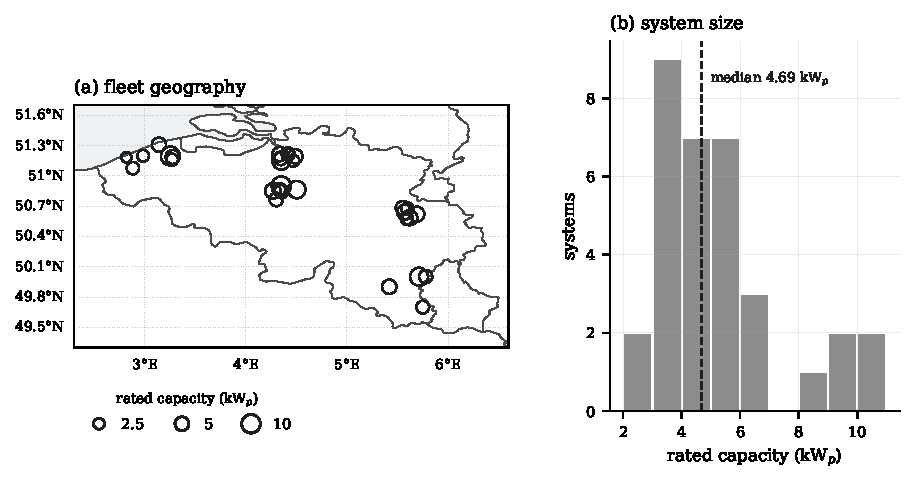
\includegraphics[width=\textwidth]{figures/fig1_fleet.pdf}
\caption{Study fleet. (a) Location of the 33 systems; marker area is proportional to rated capacity. (b) Distribution of rated capacity.}
\label{fig:fleet}
\end{figure}

\subsection{Installation metadata}
\label{sec:data-meta}

Owner-reported tilt, azimuth, rated capacity and inverter rating all enter the model (Section~\ref{sec:methods}), and none survives inspection intact (Fig.~\ref{fig:metadata}). Nine systems report a tilt of 1$^\circ$ or less, three of them exactly 0$^\circ$. Nine flat roofs in a sample of 33 Belgian houses is implausible, and the round values indicate unfilled fields. \citet{Killinger2018} filtered such entries; our pipeline used them as reported, so the transposition for these nine systems uses a near-horizontal plane. Azimuth is recorded only as a compass sector and takes three values: south (17 systems), south-west (9) and south-east (7). No east- or west-facing roof is present, and 180$^\circ$ stands for both a true southern aspect and an unreported one.

Rated capacity has the subtler problem. The ratio of each system's 99th-percentile output, $P_{99}$, to its nameplate capacity $C_\mathrm{p}$ has median 0.794 and range 0.568--1.273, a 2.24-fold spread in what full output means. Inverter clipping does not explain it, although DC capacity exceeds the inverter rating for 26 systems. On the 31 systems with a plausible inverter rating, the capacity ratio correlates with the inverse DC/AC ratio at only +0.17, and normalising by inverter rating instead of nameplate raises the coefficient of variation of $P_{99}$ from 0.157 to 0.342.
%% Clipping test reproduced from exp5_loso_per_system.csv + systems_metadata.csv; 100651 (330 W inverter entry) and 73542 (no rating) excluded.

\begin{figure}[!htb]
\centering
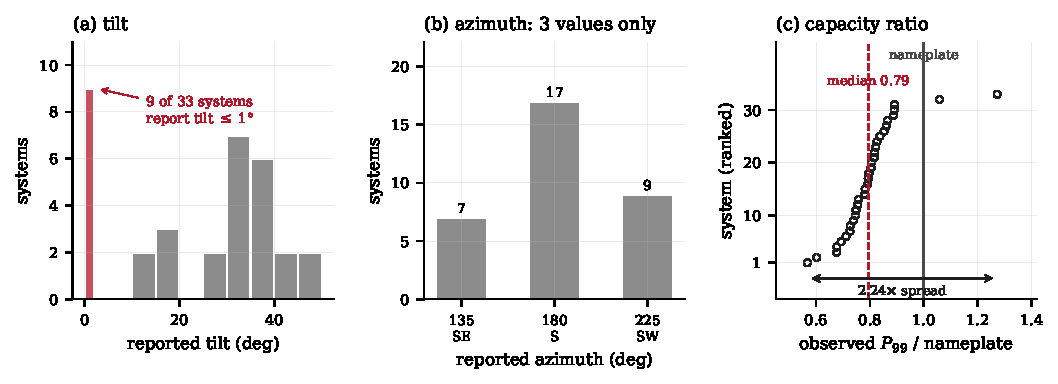
\includegraphics[width=\textwidth]{figures/fig2_metadata.pdf}
\caption{Metadata quality. (a) Reported tilt; nine systems report 1$^\circ$ or less (highlighted). (b) Reported azimuth takes three values. (c) Observed $P_{99}$ relative to nameplate capacity, ranked.}
\label{fig:metadata}
\end{figure}

\subsection{Weather forecasts}
\label{sec:data-nwp}

Day-ahead forecasts come from the Open-Meteo archive of operational NWP, retrieved with the \texttt{previous\_day1} suffix so that each value is the forecast issued one day before the target. The archive also holds analysis fields, which would be unavailable to a real forecast; none enters the features. The primary model is ECMWF IFS at 0.25$^\circ$. DWD ICON, NOAA GFS, M\'et\'eo-France, DMI and the UK Met Office supply the same variables at the same lead time, with full coverage except the Met Office (83.4\%). Seven successive ECMWF runs (\texttt{previous\_day1} to \texttt{previous\_day7}) form a lagged ensemble.

Hourly irradiance is mapped to the 15-min grid through the clear-sky index. GHI is divided by modelled clear-sky GHI with a 1~W\,m$^{-2}$ guard against division by zero, the index is interpolated linearly, and the result is multiplied by the 15-min clear-sky value. This keeps the shape of the solar curve, which direct interpolation of irradiance would flatten. The choice of clear-sky model affects downstream results \citep{Yang2020a}; we use Ineichen--Perez \citep{Ineichen2002} through pvlib \citep{Holmgren2018}.

\subsection{Reference irradiance}
\label{sec:data-ref}

Irradiance forecasts are scored against two references. ERA5 \citep{Hersbach2020} follows common practice in distributed-PV studies. SARAH-3 \citep{Pfeifroth2024,Pfeifroth2023} is the independent reference (Section~\ref{sec:rw-reference}), with 99.2\% coverage over the study window. No ground pyranometer is available for this fleet.

\subsection{Data splits}
\label{sec:data-splits}

The data are split chronologically: training from 1 April 2024 to 11 September 2025 (810,614 records), validation to 14 February 2026 (173,702) and test to 31 May 2026 (173,695). Validation is used only for hyperparameter selection and recalibration, never for reporting. Every system appears in all three partitions, so this split measures a fleet already under management and is an upper bound for a new installation. Deployment is measured separately by leave-one-system-out evaluation (Section~\ref{sec:meth-loso}).

\section{Methodology}
\label{sec:methods}

Fig.~\ref{fig:workflow} shows the inputs, the model and the three evaluation settings. The fleet oracle and the MOS branch are diagnostic arms and are never part of a deployed configuration.

\begin{figure}[!htb]
\centering
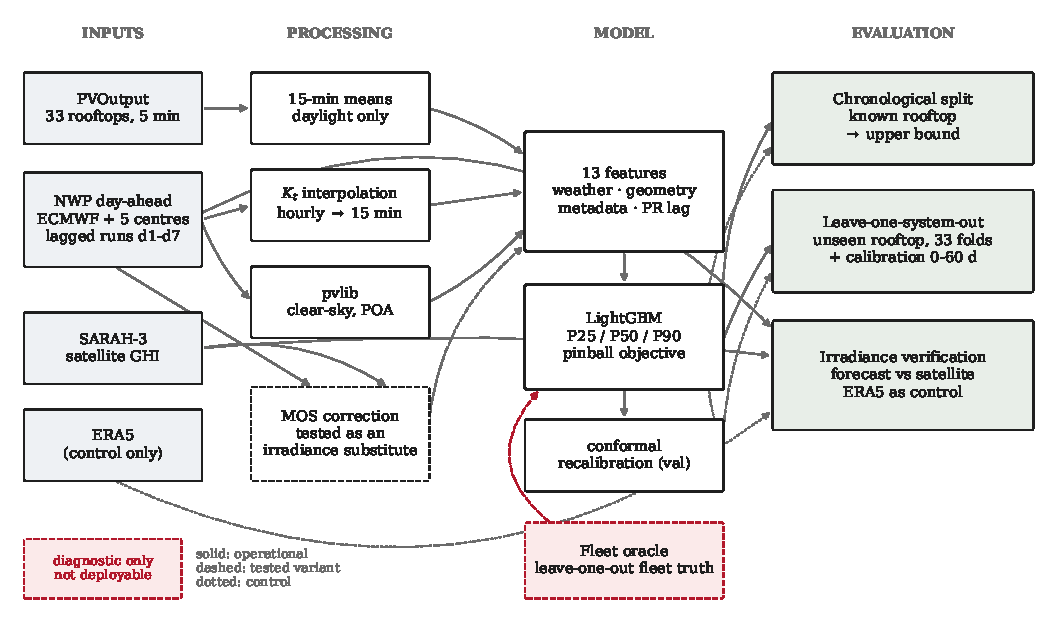
\includegraphics[width=\textwidth]{figures/fig3_workflow.pdf}
\caption{Methodology. Solid paths are operational: every input exists at the noon issue time of the preceding day. The dashed MOS branch supplies corrected irradiance as a substitute input. The shaded fleet oracle uses information unavailable at forecast time. ERA5 enters only as a control reference.}
\label{fig:workflow}
\end{figure}

\subsection{Forecast task and baseline}
\label{sec:meth-task}

For each system and each 15-min daylight slot of the following day, the model predicts output normalised by rated capacity,
\begin{equation}
y = P / (1000\,C_\mathrm{p}),
\end{equation}
with $P$ the AC output in W and $C_\mathrm{p}$ the rated DC capacity in kW$_\mathrm{p}$, clipped to $[0, 1.2]$ because real systems briefly exceed nameplate in cold, bright conditions. Normalisation lets systems of different size be learned jointly. The forecast is issued around noon of the preceding day and uses only information available then. The reference forecast is persistence, the same slot one day earlier, and skill is
\begin{equation}
S = 1 - \mathrm{RMSE}_\mathrm{model} / \mathrm{RMSE}_\mathrm{persistence}.
\end{equation}
Skill is the headline metric (Section~\ref{sec:rw-prob}). Because part of the previous day is not yet observed at noon, this persistence is slightly optimistic, so the reported skill is conservative.

\subsection{Features}
\label{sec:meth-features}

Thirteen features enter the final model (Table~\ref{tab:features}). Plane-of-array irradiance uses the Hay--Davies transposition \citep{Hay1979} in pvlib \citep{Holmgren2018} with the reported tilt and azimuth. The only site-specific history is a lagged performance ratio,
\begin{equation}
pr = y \,/\, \max(\mathrm{GHI}_\mathrm{cs}/1000,\; 0.05),
\end{equation}
taken at the same slot two days earlier, because the previous day is incomplete at noon. Lagging the ratio rather than raw output carries persistent site properties such as shading, soiling and derating, without letting yesterday's weather bias tomorrow's forecast. All NWP features are issued before the noon cutoff, so no feature uses information unavailable at issue time.

\begin{table}[!htb]
\centering
\caption{The thirteen model features. Source: E, ECMWF IFS day-ahead; I, DWD ICON day-ahead; M, mean of six centres; G, solar geometry; R, owner-reported record; H, the rooftop's own history.}
\label{tab:features}
\small
\begin{tabularx}{\textwidth}{@{}r X l l@{}}
\toprule
\# & Feature & Unit & Src \\
\midrule
1 & Plane-of-array irradiance (ECMWF) & W\,m$^{-2}$ & E \\
2 & Plane-of-array irradiance (ICON) & W\,m$^{-2}$ & I \\
3 & Clear-sky GHI, Ineichen--Perez & W\,m$^{-2}$ & G \\
4 & Direct normal irradiance & W\,m$^{-2}$ & E \\
5 & Total cloud cover & \% & I \\
6 & Multi-model mean GHI (ECMWF, ICON, GFS, M\'et\'eo-France, DMI, UK Met Office) & W\,m$^{-2}$ & M \\
7 & Solar elevation & $^\circ$ & G \\
8 & Solar azimuth & $^\circ$ & G \\
9 & $\cos(2\pi \cdot \text{minute of day} / 1440)$ & -- & G \\
10 & Rated DC capacity & kW$_\mathrm{p}$ & R \\
11 & Array tilt & $^\circ$ & R \\
12 & Array azimuth & $^\circ$ & R \\
13 & Performance ratio, same slot two days earlier & -- & H \\
\bottomrule
\end{tabularx}
\end{table}

\subsection{Model and hyperparameter selection}
\label{sec:meth-model}

Forecasts come from LightGBM gradient-boosted trees \citep{Ke2017,Friedman2001}. One model is fitted for each quantile $\alpha \in \{0.25, 0.50, 0.90\}$, each minimising the pinball loss
\begin{equation}
L_\alpha(y, \hat{y}) = \max\left[\alpha (y - \hat{y}),\; (\alpha - 1)(y - \hat{y})\right],
\end{equation}
whose minimiser is the conditional $\alpha$-quantile \citep{Koenker1978}. P50 serves as the point forecast. Predictions are clipped to $[0, 1.2]$.

Two hyperparameter searches use a tree-structured Parzen estimator in Optuna \citep{Akiba2019}, each for a different population.

\textbf{Temporal search (known rooftops).} Sixty trials per quantile minimise the pinball loss at that quantile on the validation split. Within the training split, the first 85\% fits the trees and the last 15\% sets early stopping, so the stopping rule and the selection never share data. The comparison is a preliminary configuration selected by 20 trials minimising validation RMSE under squared error and reused for all quantiles (experiment E0).

\textbf{Transfer search (unseen rooftops).} The inner loop holds out whole systems instead of future dates. The systems of a 45\% row subsample of the training and validation periods are split into three folds of eleven. Each trial trains on two folds and is scored by P50 pinball loss on the held-out systems, with early stopping on a time-tail of the training systems. Forty trials were run for P50 only.

The temporal configuration is used for every experiment on the chronological split; the transfer configuration is used for P50 in every leave-one-system-out experiment. The two are never compared as interchangeable.

\subsection{Ensemble constructions}
\label{sec:meth-ens}

Three ways of widening the weather input are compared, all at a day-ahead lead time. A \emph{lagged ensemble} averages ECMWF runs issued one to seven days before the target. A \emph{multi-model ensemble} averages the day-ahead GHI of the six centres, ignoring missing members (feature 6). \emph{Ensemble dispersion} supplies the standard deviation across all twelve members, across lagged members and across centres, the interquartile range and the fraction of members within $\pm 15\%$ of the mean.

\subsection{Fleet oracle}
\label{sec:meth-oracle}

To bound the value of perfect regional weather knowledge, the oracle feature for system $i$ at time $t$ is the mean measured output of all other systems at the same instant,
\begin{equation}
o(i, t) = \frac{\sum_j y(j, t) - y(i, t)}{n(t) - 1},
\end{equation}
with $n(t)$ the number of systems reporting, and used only where $n(t) > 3$. Thirty-three rooftops across Belgium form a distributed irradiance sensor network, so $o(i,t)$ is a close proxy for what the regional sky did. Three arms are compared on identical rows: the baseline features, the baseline plus the oracle, and the oracle with solar geometry and metadata but no NWP.

\subsection{Verification and recalibration}
\label{sec:meth-verif}

Point accuracy is reported as MAE, RMSE, mean bias error (MBE, observed minus predicted, so positive means under-forecasting), $R^2$ and skill. Irradiance bias is reported as forecast minus reference, so positive means over-forecasting, following \citet{Tuononen2019}. Probabilistic quality is reported as the mean pinball loss over the three quantiles, a proper score \citep{Gneiting2007}, as reliability, the empirical frequency of observations below each quantile \citep{Lauret2019}, and as coverage of the P25--P90 band against its nominal 0.65. Errors are stratified by the \emph{forecast} clear-sky index, which is known when decisions are made. Stratifying by the observed index conditions on the target and makes $R^2$ uninterpretable within bins, so only RMSE and bias are read from that view.

Raw quantile regression under-covers at the tails. A conformal-style offset \citep{Romano2019} is fitted on the validation split and applied unchanged to the test split,
\begin{equation}
\delta_q = \mathrm{Quantile}_q\!\left(y_\mathrm{val} - \hat{y}_{\mathrm{val},q}\right), \qquad \hat{y}_{\mathrm{test},q} \leftarrow \mathrm{clip}\!\left(\hat{y}_{\mathrm{test},q} + \delta_q,\; 0,\; 1.2\right).
\end{equation}

\subsection{Model output statistics}
\label{sec:meth-mos}

MOS is tested in two stages. At the \emph{irradiance stage}, a model learns the forecast error, truth minus ECMWF GHI, from ten predictors available at issue time: ECMWF GHI, cloud cover and temperature, clear-sky GHI, the forecast clear-sky index, solar elevation, and sine--cosine pairs of time of day and day of year. Ridge regression, random forest, LightGBM and XGBoost are compared. Two arms differ only in the truth: SARAH-3 or ERA5.

At the \emph{power stage}, the corrected irradiance enters the PV model. Because the correction becomes an input, it is produced out of fold: training rows are corrected by models fitted on the other four of five chronological folds, and validation and test rows by a model fitted on the full training split. The correction is applied to the 15-min GHI and plane-of-array irradiance as a ratio, which preserves night-time zeros and the daily shape.

\subsection{Leave-one-system-out and local calibration}
\label{sec:meth-loso}

Each system is held out in turn. A model trained on the other 32 systems over the training and validation periods predicts the held-out system's test window, giving 33 zero-shot results. The first $N \in \{3, 7, 14, 30, 45, 60\}$ days of that window then fit a local correction, and the rest is scored. Four corrections are compared: none; a \emph{bias} offset equal to the mean residual; \emph{linear} rescaling, $y \approx a + b\hat{y}$; and \emph{capacity + bias}, which first rescales by the observed capacity relative to the fleet,
\begin{equation}
s = \frac{P_{99,\mathrm{cal}} / C_\mathrm{p}}{\mathrm{median}_\mathrm{fleet}\left(P_{99} / C_\mathrm{p}\right)}, \qquad s \in [0.4, 2.5],
\end{equation}
with the fleet median taken from training systems only, and then removes the residual offset. The evaluation window shrinks and moves later in the season as $N$ grows, so corrections are compared only at equal $N$.

\subsection{Experiments}
\label{sec:meth-exp}

Table~\ref{tab:experiments} lists the experiments. Each varies one factor and holds the rest fixed. All numbers in Section~\ref{sec:results} were produced by a single driver with the quantile objective, the final feature build, the splits of Section~\ref{sec:data-splits} and SARAH-3 for irradiance scoring. Computations used Python 3.12, LightGBM 4.6.0, scikit-learn 1.9.0, pandas 3.0.3 and pvlib on a 12-core workstation. The Supplementary material gives the selected hyperparameters, full result tables and computation details.

\begin{table}[!htb]
\centering
\caption{Experiments. Split: T, chronological; L, leave-one-system-out.}
\label{tab:experiments}
\small
\begin{tabularx}{\textwidth}{@{}l >{\raggedright\arraybackslash}X >{\raggedright\arraybackslash}X l@{}}
\toprule
ID & Question & Varied & Split \\
\midrule
E0 & Does the selection objective matter? & RMSE vs pinball selection & T \\
E1 & What is perfect regional weather worth? & oracle; NWP present or absent & T \\
E2 & Where does the residual error live? & stratification only & T \\
E3 & Which input widening helps? & feature subset (7 arms) & T \\
E4 & What is the proposed configuration worth? & ensemble feature; system 81376; recalibration & T \\
E5 & What does an unseen rooftop receive? & held-out system; calibration window and method & L \\
MOS & Does irradiance correction reach power? & raw or corrected irradiance & T, L \\
\bottomrule
\end{tabularx}
\end{table}

\section{Results}
\label{sec:results}

\subsection{Where the limit lies}
\label{sec:res-limit}

\textbf{Selection objective (E0).} Selecting hyperparameters under the pinball loss instead of RMSE lowers mean pinball loss from 0.02545 to 0.02529 ($-0.66\%$) and MAE from 0.0682 to 0.0673 ($-1.4\%$), and raises skill from 0.4311 to 0.4351. The gain sits where theory puts it: pinball loss falls 1.4\% at P50 and 0.45\% at P90 and rises 0.1\% at P25. Squared error targets the conditional mean, so the preliminary configuration suited the tails least. The skill gain, +0.0040, is about 60\% of what the ensemble feature adds (+0.0065; Section~\ref{sec:res-widening}).

\textbf{Fleet oracle (E1).} Adding the contemporaneous output of every other rooftop raises $R^2$ from 0.7998 to 0.8226 and skill from 0.4194 to 0.4535 (Fig.~\ref{fig:ceiling}a). Perfect regional weather knowledge is therefore worth 0.0228 in $R^2$. With the oracle, geometry and metadata but no NWP, the model reaches $R^2$ 0.7076 and skill 0.2983. Knowing what the regional sky did recovers most of what the operational model achieves; NWP adds about 0.09 in $R^2$ beyond it. Regional-scale weather information is thus largely extracted already, and what remains unexplained is not regional.

\textbf{Residual structure (E2).} Residual autocorrelation is 0.715 at 15~min, 0.556 at 30~min, 0.407 at 1~h and 0.236 at 2~h, and falls to 0.015 at 24~h (Fig.~\ref{fig:ceiling}b). An error that is smooth over hours and uncorrelated from day to day is neither bias nor noise. It is the signature of a cloud field displaced in time or space. It also explains why persistence-based and day-to-day bias corrections fail here: yesterday's error says almost nothing about today's.

\begin{figure}[!htb]
\centering
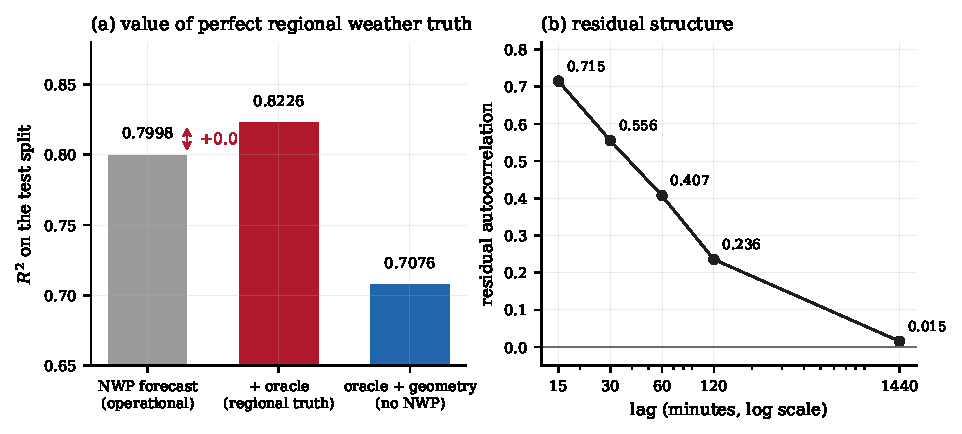
\includegraphics[width=\textwidth]{figures/fig4_ceiling.pdf}
\caption{(a) Test $R^2$ of the operational features, the same plus the fleet oracle, and the oracle without NWP. (b) Residual autocorrelation against lag.}
\label{fig:ceiling}
\end{figure}

\subsection{Where the error lives}
\label{sec:res-location}

Accuracy depends strongly on cloud (Fig.~\ref{fig:error}a). Binned by forecast clear-sky index, $R^2$ is 0.847 for clear slots ($n = 97{,}845$), but 0.440 in the 0.2--0.4 band and 0.480 in the 0.4--0.6 band. Overcast slots give 0.572 on a target standard deviation of only 0.063. Clear skies supply more than half the daylight slots and carry the pooled score; in broken cloud, where a storage controller most needs accuracy, the model explains under half the variance. Binning by the observed index reverses the sign of the conditional bias (overcast MBE +0.009 by forecast bins, $-0.068$ by observed bins), which matters when comparing with studies that condition on observed sky.

The irradiance forecast shows the same pattern against SARAH-3 (Fig.~\ref{fig:error}b). Absolute error is largest in partly cloudy conditions (RMSE 101.2~W\,m$^{-2}$) and smallest under overcast (54.9~W\,m$^{-2}$), but relative to available light the order reverses: nMAE is 36.8\% overcast, 32.4\% partly cloudy and 13.3\% clear.

The error belongs to the weather model, not to the rooftop (Fig.~\ref{fig:error}c). Across 31 rooftops spanning about $180 \times 210$~km, the ratio of the standard deviation to the median of irradiance RMSE is 0.033 in partly cloudy conditions, 0.029 in clear and 0.080 in overcast. An error driven by shading, orientation or microclimate would vary across two degrees of latitude. This one does not, so no per-rooftop feature or local calibration can remove it.

\begin{figure}[!htb]
\centering
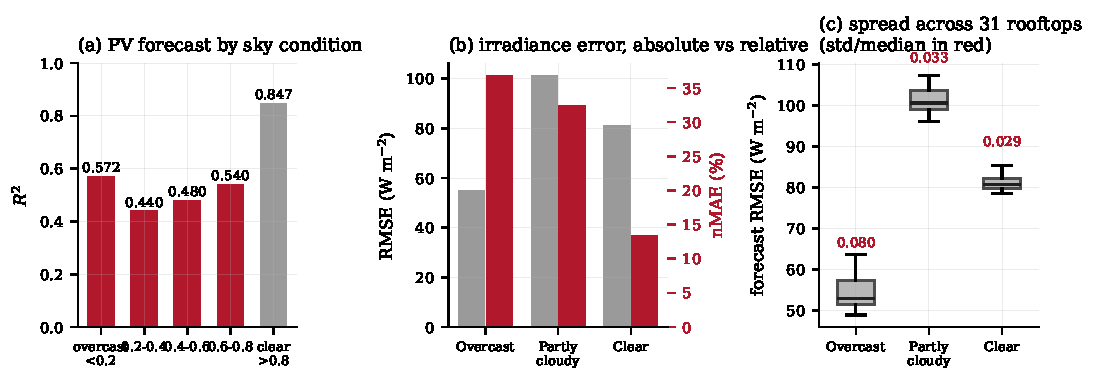
\includegraphics[width=\textwidth]{figures/fig5_error_location.pdf}
\caption{(a) PV forecast $R^2$ by forecast clear-sky index. (b) Irradiance forecast error against SARAH-3, absolute (RMSE) and relative (nMAE). (c) Per-rooftop irradiance RMSE across 31 systems.}
\label{fig:error}
\end{figure}

\subsection{Widening the weather input}
\label{sec:res-widening}

Table~\ref{tab:ablation} gives the ensemble ablation (E3). Only the multi-model mean improves every metric: skill rises from 0.4285 to 0.4351 and pinball loss falls from 0.02558 to 0.02529. Averaging ECMWF's own runs from one to three days before the target gives skill 0.4291, within noise of the baseline. Re-runs of one model are staler but not independent; centres differ in physics and therefore in error. Ensemble dispersion as a predictor lowers skill (0.4280), raises pinball loss by 1.6\% and lowers P25--P90 coverage from 0.622 to 0.592. The quantile model already infers conditional uncertainty from the clear-sky index and solar geometry, so dispersion adds mostly noise. All ten ensemble features together give a slightly higher $R^2$ but worse pinball loss and the lowest coverage (0.590).

\begin{table}[!htb]
\centering
\caption{Ensemble ablation on the chronological split, 32 systems.}
\label{tab:ablation}
\small
\begin{tabularx}{\textwidth}{@{}X c c c c@{}}
\toprule
Feature set & Features & $R^2$ & Skill & Pinball \\
\midrule
Base & 12 & 0.8070 & 0.4285 & 0.02558 \\
\textbf{+ multi-model mean (6 centres)} & 13 & \textbf{0.8114} & \textbf{0.4351} & \textbf{0.02529} \\
+ mean of all 12 members & 13 & 0.8078 & 0.4298 & 0.02552 \\
+ ensemble-mean POA & 13 & 0.8081 & 0.4301 & 0.02554 \\
+ lagged mean (ECMWF, days 1--3) & 13 & 0.8074 & 0.4291 & 0.02559 \\
+ ensemble spread only & 17 & 0.8066 & 0.4280 & 0.02598 \\
+ all 10 ensemble features & 22 & 0.8089 & 0.4314 & 0.02582 \\
\bottomrule
\end{tabularx}
\end{table}

\subsection{Proposed configuration and calibration}
\label{sec:res-config}

Table~\ref{tab:ablation} uses 32 systems because one rooftop was excluded (E4). With all 33 systems and no ensemble feature, $R^2$ is 0.7960 and skill 0.4139. Excluding system 81376 raises $R^2$ by 0.0110; adding the ensemble feature raises it by a further 0.0044, to 0.8114 (skill 0.4351). Two-thirds of the total gain comes from removing one rooftop. System 81376 holds 3.08\% of test rows but 7.69\% of squared error. Its defect is time-varying: in April--May 2026, inside the test window, its output relative to the fleet median fell to 0.60, against 0.85 and 0.89 in the same months of 2024 and 2025. This 31\% drop is the largest in the fleet (median $-3\%$), so no capacity value fixed during training can absorb it.
%% Source: v3_ensemble/src/eval/system_drift.py (season-matched April-May comparison).

Raw quantiles are over-confident at the upper tail: empirical coverage of the nominal P90 is 0.869 (Fig.~\ref{fig:recal}). Three offsets fitted on validation ($+0.0004$, $+0.0022$ and $+0.0105$ for P25, P50 and P90) bring coverage to 0.263, 0.520 and 0.912 against nominal 0.25, 0.50 and 0.90. Mean pinball loss is unchanged (0.02529 to 0.02527), and P25--P90 coverage moves from 0.614 to 0.649 against the nominal 0.65. The small over-coverage at P90 reflects validation-to-test drift and errs on the safe side for storage scheduling.

\begin{figure}[!htb]
\centering
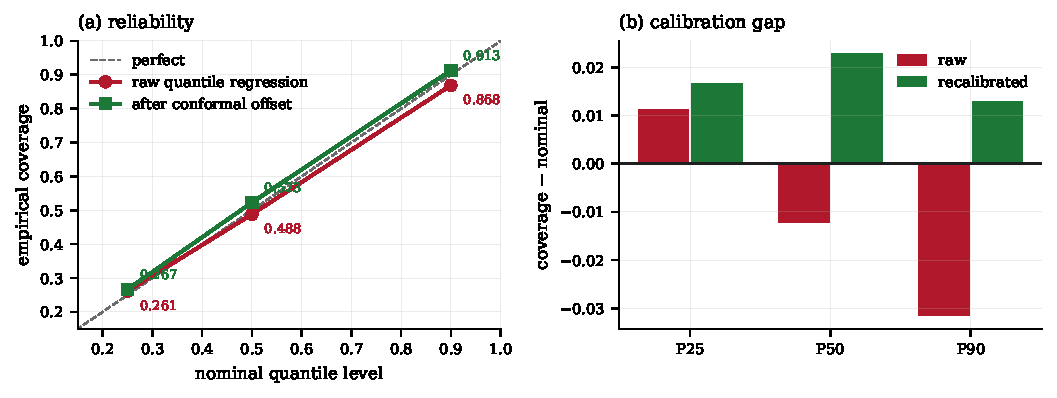
\includegraphics[width=\textwidth]{figures/fig7_recalibration.pdf}
\caption{Reliability of the proposed configuration before and after recalibration. (a) Empirical against nominal coverage. (b) Calibration gap per quantile.}
\label{fig:recal}
\end{figure}

\subsection{Irradiance correction and the reference}
\label{sec:res-mos}

\textbf{Reference.} Over the study window, the same ECMWF forecast scored against ERA5 has RMSE 51.1~W\,m$^{-2}$ and bias $-1.5$~W\,m$^{-2}$; against SARAH-3 it has 86.6~W\,m$^{-2}$ and $+9.2$~W\,m$^{-2}$. ERA5 understates RMSE by a factor of 1.69 (relative RMSE 16.5\% against 29.0\%) and reverses the sign of the bias. An external check supports the satellite figure: its bias is close to the +8~W\,m$^{-2}$ that \citet{Tuononen2019} measured for ECMWF IFS with ground instruments over four years at a comparable latitude.
%% Source: v3_ensemble/src/eval/reference_comparison.py (253,419 hourly rows, 31 systems; RMSE 86.63 vs 51.14, rRMSE 28.99 vs 16.52).

\textbf{Irradiance stage.} Against SARAH-3, random forest lowers MAE from 55.49 to 51.96~W\,m$^{-2}$ ($-6.4\%$) and RMSE from 86.27 to 81.94~W\,m$^{-2}$, raising $R^2$ from 0.866 to 0.879. Ridge regression barely changes MAE ($-0.5\%$) but cuts the bias from +11.40 to +0.88~W\,m$^{-2}$, which shows the bias is systematic. LightGBM and XGBoost make MAE worse ($-0.6\%$ and $-1.9\%$). Against ERA5, every learner degrades the forecast (MAE $-1.0\%$ to $-9.6\%$), because the raw bias against ERA5 is only +0.81~W\,m$^{-2}$ and there is nothing to learn. Trained against a reanalysis from the same model, MOS appears ineffective for the wrong reason.

\textbf{Power stage, seen rooftops.} The out-of-fold correction lowers test MAE from 55.49 to 52.13~W\,m$^{-2}$ ($-6.1\%$) and bias from +11.40 to +3.12~W\,m$^{-2}$ ($-73\%$). In the PV model it changes $R^2$ from 0.8114 to 0.8111 and skill from 0.4351 to 0.4346, and raises pinball loss from 0.02529 to 0.02539. Adding the correction as two extra features instead is slightly worse (0.8109, 0.4344, 0.02549).

\textbf{Power stage, unseen rooftops.} On a rooftop absent from training, the model cannot have absorbed that rooftop's share of the bias, so MOS should matter more. It does not. Across 33 held-out rooftops the median change is +0.00012 in $R^2$ and +0.00016 in skill; 17 of 33 rooftops improve, and changes range from $-0.0166$ to $+0.0361$. The largest gains are on 94362 (+0.0361) and 81376 (+0.0196), two of the worst-transferring rooftops, where the irradiance correction partly offsets a capacity error (Section~\ref{sec:res-deploy}); neither becomes usable. After 30 days of capacity + bias calibration, median skill is 0.3281 with MOS and 0.3230 without.

The reason is proportion. MOS removes about 8~W\,m$^{-2}$ of systematic bias, but RMSE falls only from 86.3 to 82.2~W\,m$^{-2}$. The remainder is the displacement error of Section~\ref{sec:res-limit}, which no statistical bias correction can reach, and the PV model has already fitted around the systematic part.

\subsection{Deployment on an unseen rooftop}
\label{sec:res-deploy}

A rooftop absent from training receives median $R^2$ 0.704 and skill 0.347, against 0.811 and 0.435 pooled over known rooftops on the chronological split. The tail matters more than the median: mean $R^2$ is 0.658, the 10th percentile 0.497 and the worst $-0.158$. Two of 33 rooftops, about one in sixteen, score worse than persistence.

\textbf{Hyperparameters for transfer.} Table~\ref{tab:transfer} and Fig.~\ref{fig:deploy} compare three configurations on the same 33 rooftops. The configuration that wins on the chronological split is the worst on unseen rooftops: mean $R^2$ 0.588, worst case $-0.985$, five failures. Selecting against held-out systems leaves the median almost unchanged but raises the 10th percentile from 0.308 to 0.496, lifts the worst rooftop to $-0.156$ and halves the failures. The transfer configuration has depth 4 and L2 penalty 4.34, against depth 15 and 0.008 for the temporal one. A depth-4 tree cannot encode rooftop identity and must learn what rooftops share.
%% Table 4 comes from tune_transfer.py (fixed seed); the E5 values above from consolidate.py (default seed). Same configuration; the 0.005 difference in median R2 is bagging-seed variation.

\begin{table}[!htb]
\centering
\caption{Zero-shot $R^2$ and skill on 33 held-out rooftops for three hyperparameter configurations. Failures: skill $\le 0$.}
\label{tab:transfer}
\small
\begin{tabularx}{\textwidth}{@{}X c c c c c c@{}}
\toprule
Configuration & Median & Mean & P10 & Worst & Median skill & Failures \\
\midrule
Preliminary (RMSE, temporal) & 0.719 & 0.603 & 0.378 & $-0.709$ & 0.293 & 4 \\
Tuned on temporal split & 0.708 & 0.588 & 0.308 & $-0.985$ & 0.316 & 5 \\
\textbf{Tuned on held-out systems} & 0.710 & \textbf{0.657} & \textbf{0.496} & $\mathbf{-0.156}$ & \textbf{0.340} & \textbf{2} \\
\bottomrule
\end{tabularx}
\end{table}

\begin{figure}[!htb]
\centering
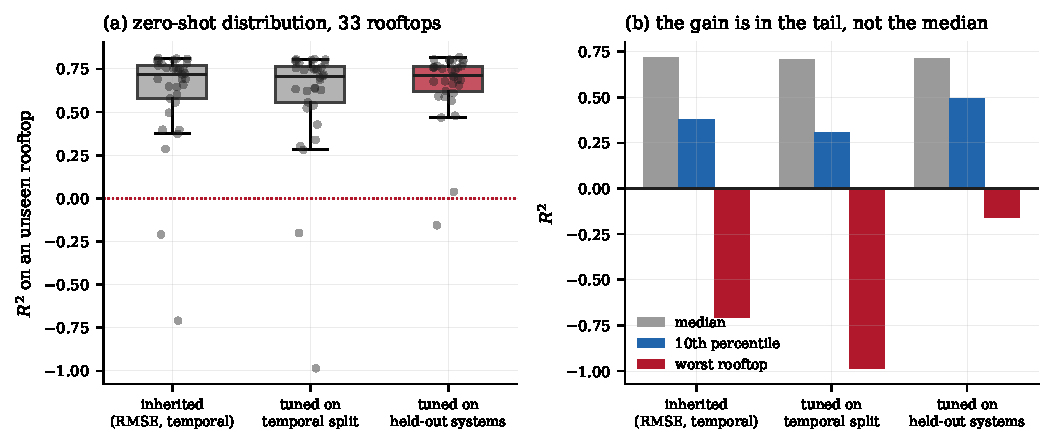
\includegraphics[width=\textwidth]{figures/fig8_deployment.pdf}
\caption{Zero-shot $R^2$ on 33 held-out rooftops for three configurations. (a) Distributions with individual rooftops. (b) Median, 10th percentile and worst case.}
\label{fig:deploy}
\end{figure}

\textbf{Rated capacity.} On unseen rooftops, the capacity ratio $P_{99}/C_\mathrm{p}$ (Section~\ref{sec:data-meta}) correlates with forecast bias at +0.709. The model learns the fleet-average relation between output and nameplate. A rooftop whose nameplate overstates its real capacity is over-forecast, and one whose nameplate understates it is under-forecast. On the chronological split this is hidden, because the model memorises each rooftop's scale. The lowest ratio in the fleet, 0.568, belongs to 94362 ($R^2$ 0.067); the worst rooftop, 81376 ($R^2$ $-0.158$), has a ratio of 0.693, also in the lowest fifth.

\textbf{Local calibration (E5).} Fig.~\ref{fig:calib} shows median skill against the length of the local window. Below about 30 days every correction is harmful: at 3 days, linear rescaling gives skill $-0.110$ against 0.347 uncorrected, because two parameters are fitted to a window that may contain no clear day. From 30 days, correction helps and linear rescaling is best, by +0.009 skill at 30 days, +0.022 at 45 and +0.053 at 60. Median $R^2$ rises from 0.704 at day 0 to 0.755 with linear rescaling at 45 days. The operating rule is no correction before 30 days of local history, then linear rescaling on a rolling window.

\begin{figure}[!htb]
\centering
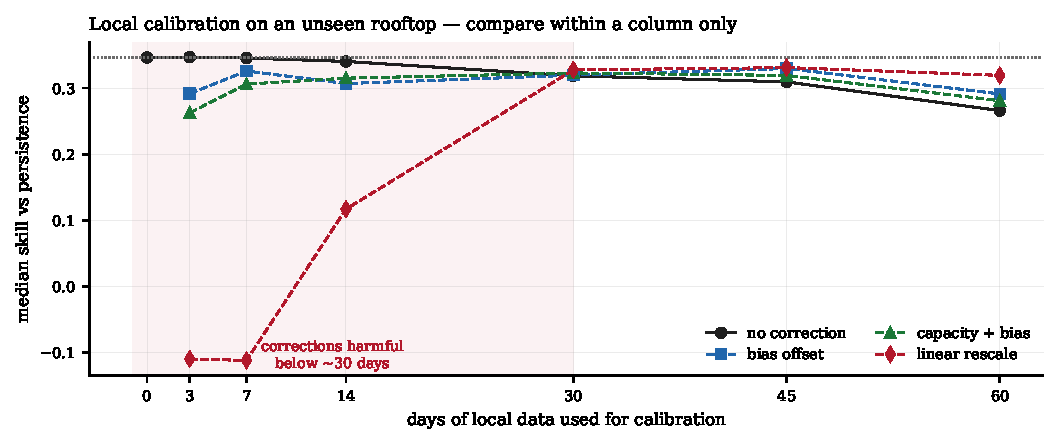
\includegraphics[width=\textwidth]{figures/fig9_calibration_sweep.pdf}
\caption{Median skill on held-out rooftops against local calibration window, by correction method. The shaded region marks where correction is harmful. Compare methods only at the same window length.}
\label{fig:calib}
\end{figure}

\subsection{Comparison with published results}
\label{sec:res-compare}

Cross-study comparison is unreliable. Accuracy depends on climate, horizon, resolution, aggregation and plant type, and on conventions: the same forecast here has normalised RMSE of 11.0\% of capacity but 38.0\% of mean output. Skill depends on the reference \citep{Yang2019}. \citet{Visser2019}, for example, report skill against smart persistence, a stronger reference than the plain persistence used here, so the two skills are not comparable. Utility-scale probabilistic results such as \citet{MayerYang2023} use a different normaliser and score. The comparisons that do hold are qualitative: tree ensembles were also the best learners on 152 distributed systems \citep{Visser2019}; input outweighs model family at day-ahead \citep{Nguyen2026}; and the 30-day calibration threshold has the same order of magnitude as the two months a local model needs in \citet{Depoortere2025}. The bias check in Section~\ref{sec:res-mos} supports the measurement chain. We do not claim higher accuracy than published work: Section~\ref{sec:res-limit} shows the accuracy of any learner here is bounded by the input.

\section{Discussion}
\label{sec:discussion}

\subsection{Post-processing and the validation reference}
\label{sec:disc-mos}

The MOS correction works at the level it was built for, and the gain then disappears in the PV model. Two causes combine. The systematic component is about a tenth of the irradiance error, so even its full removal leaves the problem intact. And a learner trained on the biased input has already fitted around that bias, so it never used the input at face value. The value of post-processing therefore depends on what consumes it. For a physical model chain, which propagates irradiance deterministically, the premise that better irradiance gives better power holds \citep{Mayer2021,Mayer2022}. For a statistical model trained on the same distribution, the gain may not survive, and only an end-to-end test shows whether it does.

The reference result has the same practical weight. Scored against ERA5, the irradiance bias almost vanishes and MOS fails under every learner; scored against SARAH-3, the same procedure works. A study that stopped at the reanalysis comparison would have reached the right outcome for the wrong reason. A reanalysis produced by the same centre with the same model as the forecast is not an independent reference, and agreement with it is not evidence of forecast quality.

\subsection{Transfer: hyperparameters and metadata}
\label{sec:disc-transfer}

Hyperparameters selected on a chronological split reward memorising individual rooftops, because those rooftops recur in the test set. On unseen rooftops this capacity becomes a liability. The finding should apply to any fleet model tuned where all units are seen and deployed where they are not. The remedy is cheap, a grouped split in the inner loop of the search, yet it is rarely reported because transfer is rarely evaluated.

For a fleet built from volunteer data, the binding constraint on deployment is the installation record, not the weather model. Excluding one defective rooftop improved $R^2$ by 0.0110, against 0.0044 for the best weather-input change, and the capacity ratio tracks bias on unseen rooftops. Two remedies follow. Tilt and azimuth can be inferred from generation data \citep{Meng2020} instead of trusted. Capacity can be estimated from observed output, but Section~\ref{sec:res-deploy} shows this needs about a month of local history. Before that, a grid operator or aggregator should screen new installations for implausible metadata before relying on their forecasts.

\subsection{What would move the limit}
\label{sec:disc-limit}

At the day-ahead horizon the constraint is the placement and timing of cloud at kilometre and minute scales, not the statistical layer. Higher-resolution NWP is the direct route; the choice of NWP source affects PV accuracy materially \citep{Mayer2023}, and convection-permitting regional models resolve cloud structure that a 0.25$^\circ$ grid cannot. Whether that resolution survives to a day-ahead forecast for a single rooftop is beyond what our data can test. Satellite nowcasting informs the next hours, not the next day.

\subsection{Limitations}
\label{sec:disc-limitations}

\begin{itemize}
\item \textbf{Fleet.} Thirty-three rooftops in one country and one NWP regime over 26 months, with no east- or west-facing system. Other climates and orientations are untested.
\item \textbf{Reference.} SARAH-3 is a retrieval with its own uncertainty (Section~\ref{sec:rw-reference}); no ground pyranometer was available.
\item \textbf{Metadata used as supplied.} The nine near-flat tilt entries were not filtered. Their median zero-shot $R^2$ (0.704) does not differ significantly from the rest of the fleet (0.723; Mann--Whitney $p = 0.53$), but their transposition is wrong. Coordinates were not perturbed, although \citet{Depoortere2025} show that location errors can remove the transfer advantage.
\item \textbf{Hyperparameter searches.} Both were budget-limited: temporal learning rates (0.013--0.015) lie near the floor of 0.010, and tree counts reached or approached their caps (2000 temporal, 1500 transfer). The transfer search covered P50 only, so the P25 and P90 models in deployment use the temporal configuration.
\item \textbf{Learner and ensemble.} Only gradient-boosted trees were tested under the final protocol. Lagged and multi-model constructions stand in for a true initial-condition ensemble, which we could not retrieve for the study window; the dispersion result may not transfer to one.
\item \textbf{Grid value.} Forecast quality is reported in statistical terms. Its effect on feeder-level operation, imbalance cost or battery scheduling is not quantified.
\end{itemize}

\section{Conclusions}
\label{sec:conclusions}

Day-ahead forecasting for individual residential rooftops is limited by the NWP input, not by the learner. Four independent tests on 33 Belgian rooftops support this:
\begin{enumerate}
\item perfect regional weather knowledge adds only 0.023 in $R^2$;
\item residuals decorrelate within a day, the signature of displaced cloud;
\item irradiance error is nearly identical across rooftops up to 210~km apart;
\item removing 73\% of the irradiance bias leaves PV accuracy unchanged on seen and unseen rooftops.
\end{enumerate}

Within that limit, gains are small. Averaging forecasts across six centres helps; averaging one centre's re-runs does not, and ensemble dispersion hurts. Recalibration gives honest P90 coverage (0.912) at no cost in accuracy.

Two results apply beyond this dataset. Validating against a reanalysis from the same model understates RMSE 1.69-fold and reverses the bias. Hyperparameters chosen where every unit is seen transfer poorly; selecting them against held-out systems halves the failures on unseen rooftops.

For grid operators and aggregators, a newly connected rooftop should be expected to perform well below chronological-split figures (median $R^2$ 0.704 against 0.811). Local calibration should wait for about 30 days of history. Transfer failures follow the installation record, chiefly rated capacity, rather than the weather. Effort is therefore better spent on higher-resolution NWP and on metadata inference and screening than on further changes of learner.


%% Declarations. Elsevier requires these sections at submission.
%% They are short; check the current guide on whether they count toward the 7000 words.

\section*{Data availability}
All analysis code (data retrieval, feature construction, model fitting, the oracle and MOS protocols, the leave-one-system-out harness and the figure scripts) is available at \url{https://github.com/DT-Service-Consulting/solcent}, tag \texttt{v1.1-paper}. The archive includes the derived outputs needed to reproduce every table and figure. Weather forecasts are retrieved from the Open-Meteo archive (CC BY 4.0); retrieval scripts are supplied instead of the fields, because upstream providers have their own terms. SARAH-3 is available from EUMETSAT CM SAF \citep{Pfeifroth2023}. PV generation data are published by system owners on PVOutput.org, whose terms do not allow redistribution. The archive therefore contains the system identifiers and the retrieval script, so that any user with PVOutput access can rebuild the dataset.

\section*{CRediT authorship contribution statement}
%% TODO: one line per author, e.g.
%% \textbf{Chandradip Roy:} Conceptualization, Methodology, Software, Formal analysis, Writing -- original draft.

\section*{Declaration of competing interest}
%% TODO: confirm. Standard wording:
The authors declare that they have no known competing financial interests or personal relationships that could have appeared to influence the work reported in this paper.

\section*{Declaration of generative AI and AI-assisted technologies in the manuscript preparation process}
%% TODO: Elsevier asks authors to declare AI tools used in writing. Edit or remove to match what you actually used.
During the preparation of this work the author(s) used [TOOL NAME] in order to [REASON]. After using this tool/service, the author(s) reviewed and edited the content as needed and take(s) full responsibility for the content of the published article.


\FloatBarrier
\bibliographystyle{elsarticle-harv}
\bibliography{refs}

\end{document}
